

\section{Gráficos}\label{sec_graf}

A \hl{\PYTHONmatplotlib} é uma biblioteca {\python} livre e gratuita para a visualização de dados. É muito utilizada para a criação de gráficos estáticos, animados ou iterativos. Aqui, vamos introduzir alguma de suas ferramentas básicas para gráficos.

Usualmente, importamos a biblioteca com

\begin{lstlisting}
import matplotlib.pyplot as plt
\end{lstlisting}

\subsection{Gráfico de uma função}\label{sec_graf_ssec_fun}

\begin{figure}[h]
  \centering
  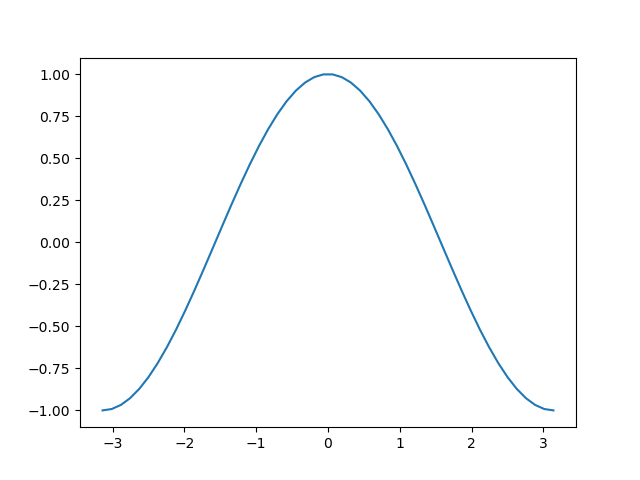
\includegraphics[width=3in]{sec_grafico/data/sen.png}
  \caption{Esboço do gráfico da função $y=\cos(x)$ no intervalo $[-\pi,\pi]$.}
  \label{fig:sen}
\end{figure}

A função {\PYTHONmatplotlibDOTpyplotDOTplot}\texttt{(x,y)} pode ser usada para criarmos gráficos, onde \texttt{x} e \texttt{y} são {\PYTHONnumpyDOTarrays} que fornecem os pontos cartesianos $\{(x_i, y_i)\}_{i}$ a serem plotados. Por exemplo,

\begin{lstlisting}
import numpy as np
import matplotlib.pyplot as plt
x = np.linspace(-np.pi, np.pi)
y = np.cos(x)
plt.plot(x,y)
plt.show()
\end{lstlisting}

produz um esboço do gráfico da função $y=\cos(x)$ no intervalo $[-\pi,\pi]$. Consulte a Figura \ref{fig:sen}.


\begin{obs}
  {\PYTHONmatplotlib} é uma poderosa ferramenta para a visualização de gráficos. Consulte a galeria de exemplos no seu site oficial
  \begin{center}
    \url{https://matplotlib.org/stable/gallery/index.html}
  \end{center}
\end{obs}

\begin{exer}
  Crie um esboço do gráfico de cada uma das seguintes funções no intervalo indicado:
  \begin{enumerate}[a)]
  \item $y = \cos(x)$, $\left[0, 2\pi\right]$
  \item $y = x^2 - x + 1$, $[-2, 2]$
  \item $y = \tg\left(\frac{\pi}{2}x\right)$, $(-1, 1)$
  \end{enumerate}
\end{exer}
\begin{resp}

a)

\begin{lstlisting}
import numpy as np
import matplotlib.pyplot as plt
x = np.linspace(0, 2*np.pi)
y = np.cos(x)
plt.plot(x, y, ls='--')
plt.show()
\end{lstlisting}

b)

\begin{lstlisting}
import numpy as np
import matplotlib.pyplot as plt
x = np.linspace(-2, 2)
plt.plot(x, x**2-x+1, color='red')
plt.grid()
plt.show()
\end{lstlisting}

c)

\begin{lstlisting}
import numpy as np
import matplotlib.pyplot as plt
x = np.linspace(-1, 1)
y = np.tan(np.pi/2*x)
plt.plot(x, y)
plt.ylim(-10, 10)
plt.xlabel('x')
plt.ylabel('y')
plt.grid()
plt.show()
\end{lstlisting}

\end{resp}

\ifisbook 
\subsubsection*{Respostas dos Exercícios}
\shipoutAnswer
\fi

